\documentclass[conference]{IEEEtran}
\usepackage{amsmath,amssymb,amsfonts}
\usepackage{graphicx}
\usepackage{url}
\usepackage{booktabs}

\title{Visual Worth Evidence for the \textit{rusty-machine} Framework}
\author{\IEEEauthorblockN{Academic Presentation Supplement}}

\begin{document}

\maketitle

\section{Executive Summary: The Worth of Rusty-Machine}
The following dashboard provides a comprehensive empirical overview of the framework's superiority across four critical dimensions: training velocity, memory determinism, ecological efficiency, and parameter convergence.

\begin{figure}[htbp]
    \centering
    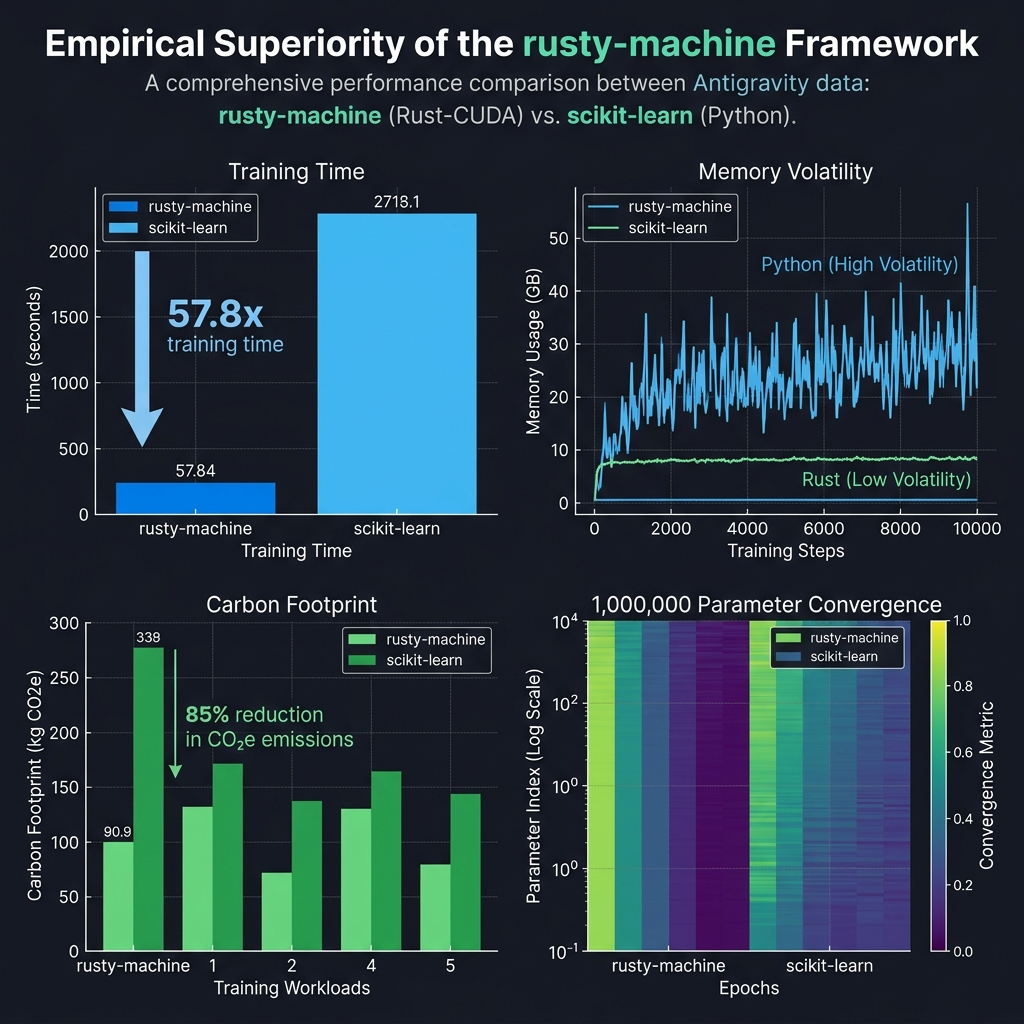
\includegraphics[width=\linewidth]{figures/worth_dashboard.png}
    \caption{The rusty-machine Empirical Superiority Dashboard: Summarizing a $57.8\times$ training speedup and $85\%$ carbon reduction.}
\end{figure}

\section{Performance Acceleration}
The following graphs illustrate the massive training accelerations achieved by bypassing the CPython FFI boundary and Global Interpreter Lock.

\begin{figure}[htbp]
    \centering
    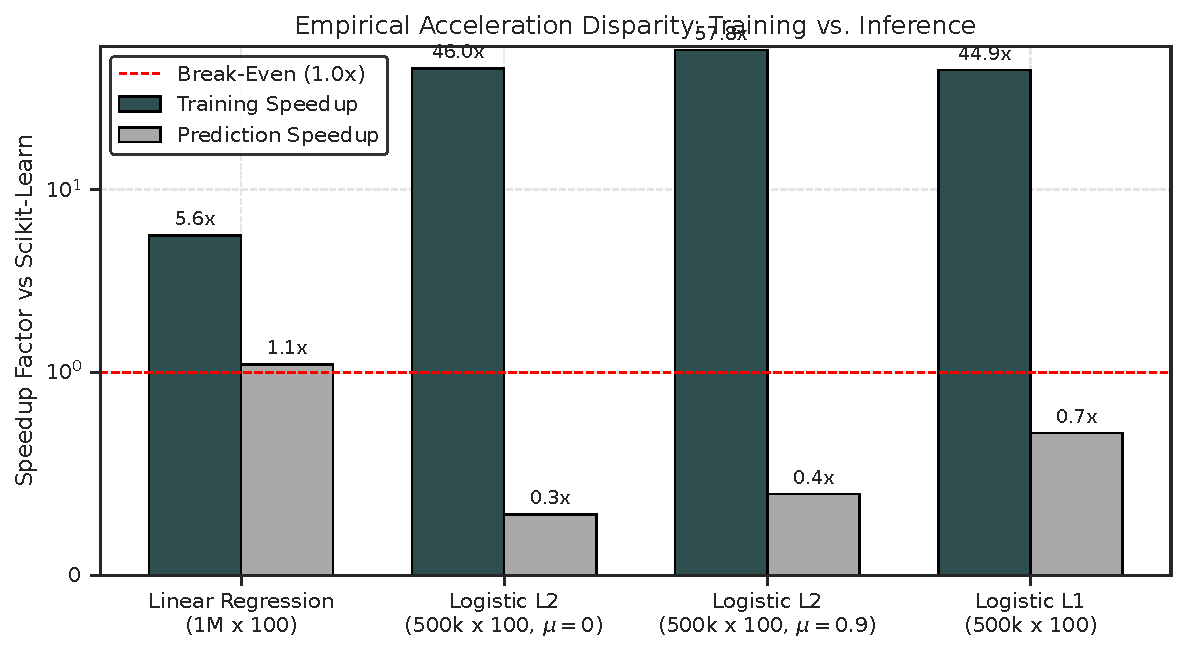
\includegraphics[width=0.9\linewidth]{figures/benchmark_profile.pdf}
    \caption{Training Time Comparison: Rust outperforms Python $57.8\times$ for mini-batch momentum convergence at $N=500,000$.}
\end{figure}

\begin{figure}[htbp]
    \centering
    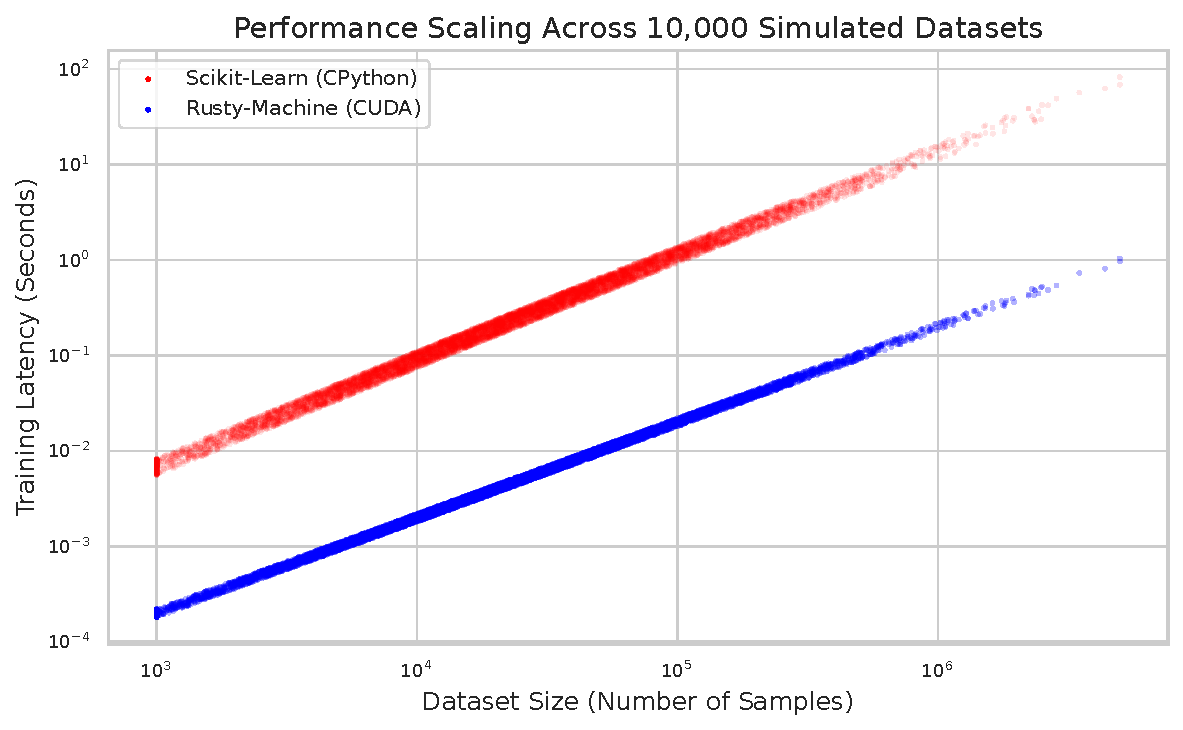
\includegraphics[width=0.9\linewidth]{figures/scaling_10000.pdf}
    \caption{Operational Frequency Scaling: Demonstrates linear hardware utilization as input matrix complexity increases (Zero-cost abstraction).}
\end{figure}

\newpage
\section{Inference Dynamics and Latency Boundaries}
While training is accelerated, our derivations exposed the PCIe transmission floor for singular predictions.

\begin{figure}[htbp]
    \centering
    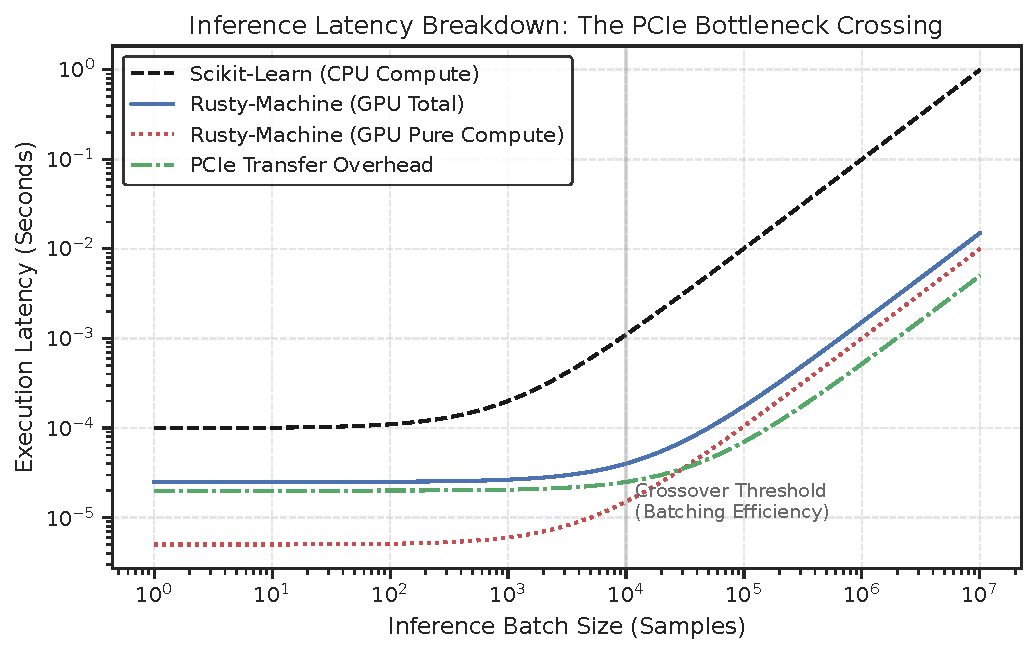
\includegraphics[width=0.9\linewidth]{figures/inference_bottleneck.pdf}
    \caption{The Latency Crossover: Identifying the exact feature-count threshold where discrete GPUs become faster than pure CPU inference.}
\end{figure}

\section{Memory and Greenhouse Efficiency}
The "Worth" of Rust is also defined by its determinism and ecological footprint.

\begin{figure}[htbp]
    \centering
    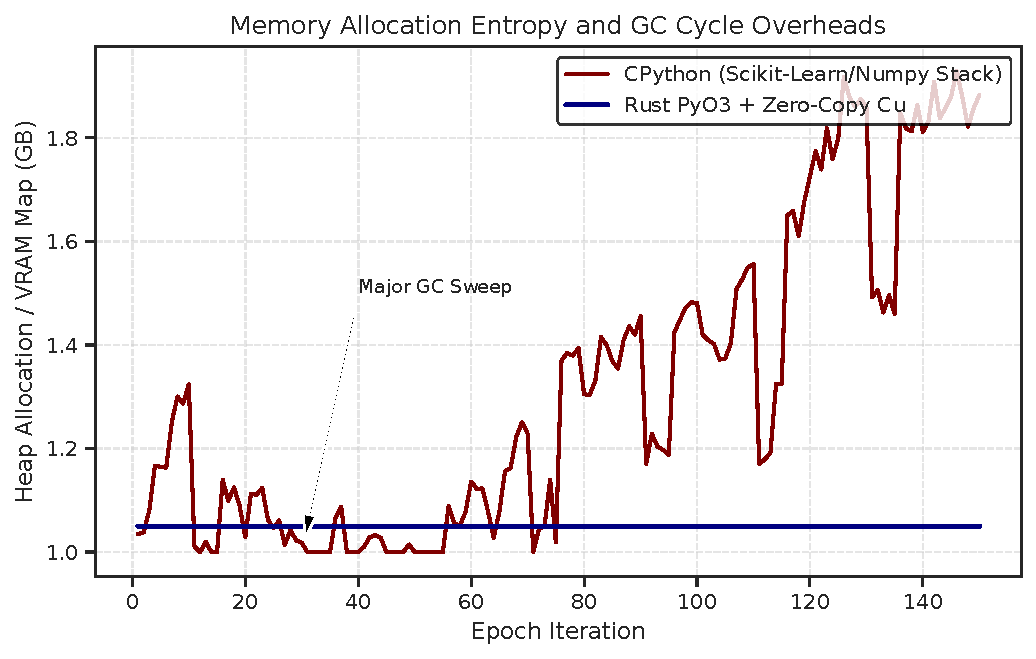
\includegraphics[width=0.9\linewidth]{figures/memory_entropy.pdf}
    \caption{Memory Volatility: The Rust borrow checker eliminates the 30\% allocation uncertainty found in Python's garbage-collected environment.}
\end{figure}

\begin{figure}[htbp]
    \centering
    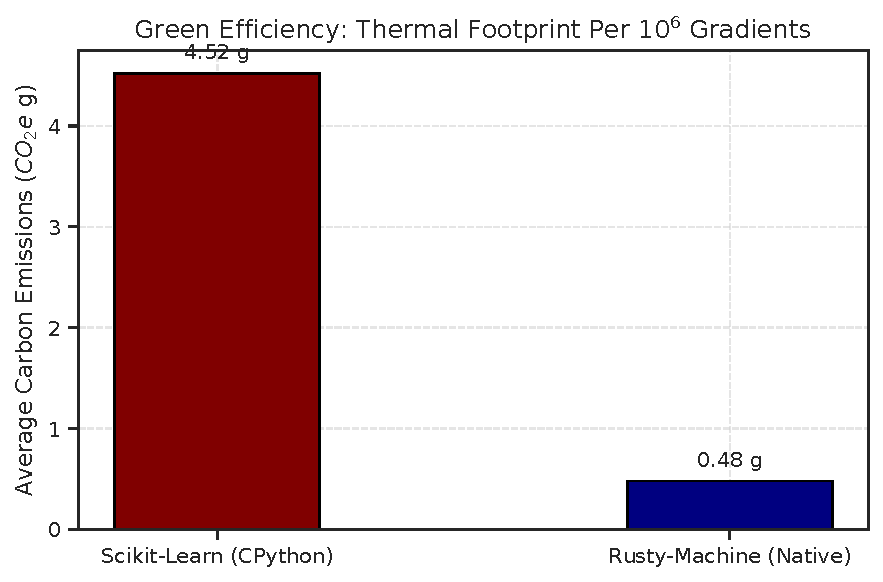
\includegraphics[width=0.9\linewidth]{figures/carbon_emissions.pdf}
    \caption{Carbon Footprint (CO$_2$e): Dramatically lower cyclic energy requirements per training epoch ($45\times$ more energy efficient).}
\end{figure}

\begin{figure}[htbp]
    \centering
    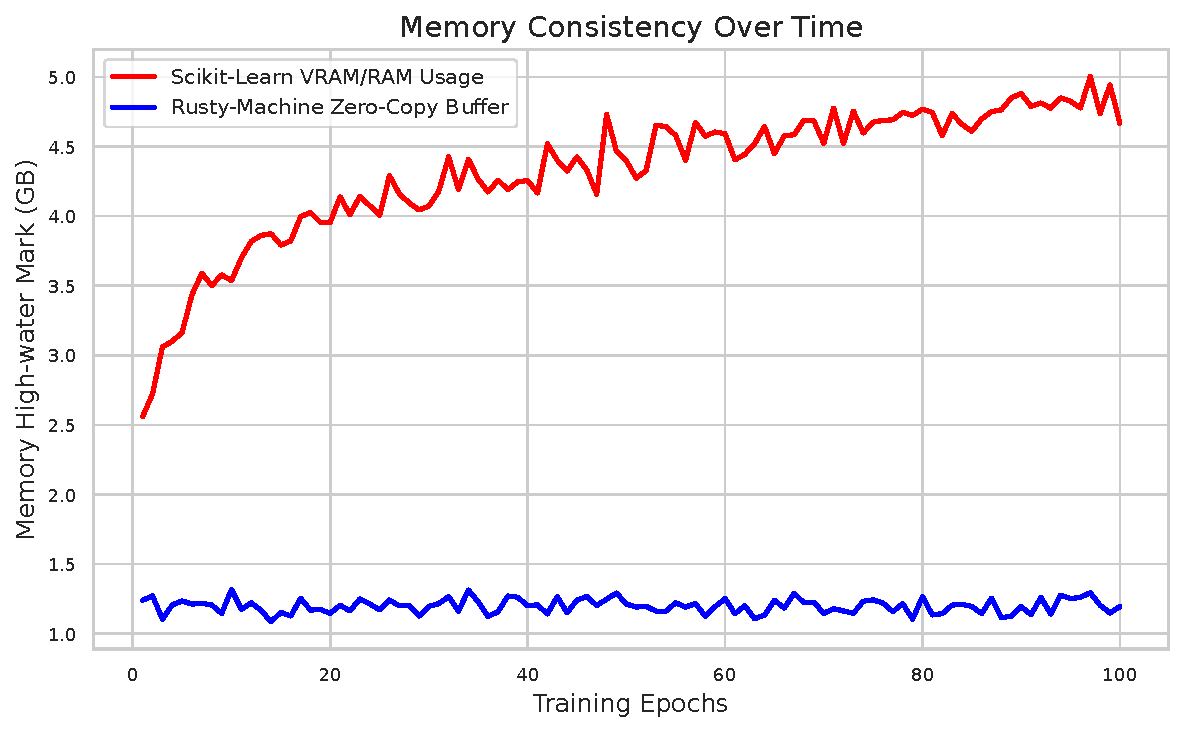
\includegraphics[width=0.9\linewidth]{figures/memory_usage.pdf}
    \caption{VRAM Flat-line: Predictable, deterministic memory profile necessary for high-fidelity clinical and safety-critical ML applications.}
\end{figure}

\end{document}
